Taking into account the goals of this project and all the technology presented so far. Our proposal is the development of a web application that provides communication and collaboration in real-time.

The requirements for our web application are:

\begin{itemize}
 \item Enrich calls with any kink of multimedia in real-time.
 \item Ability perform tasks on real-time collaborative environment.
 \item Ability to record and playback interactive multimedia.
\end{itemize}

\subsection{Modules}
	Our system is divided into five modules.

\begin{figure}[H]
	\centering
	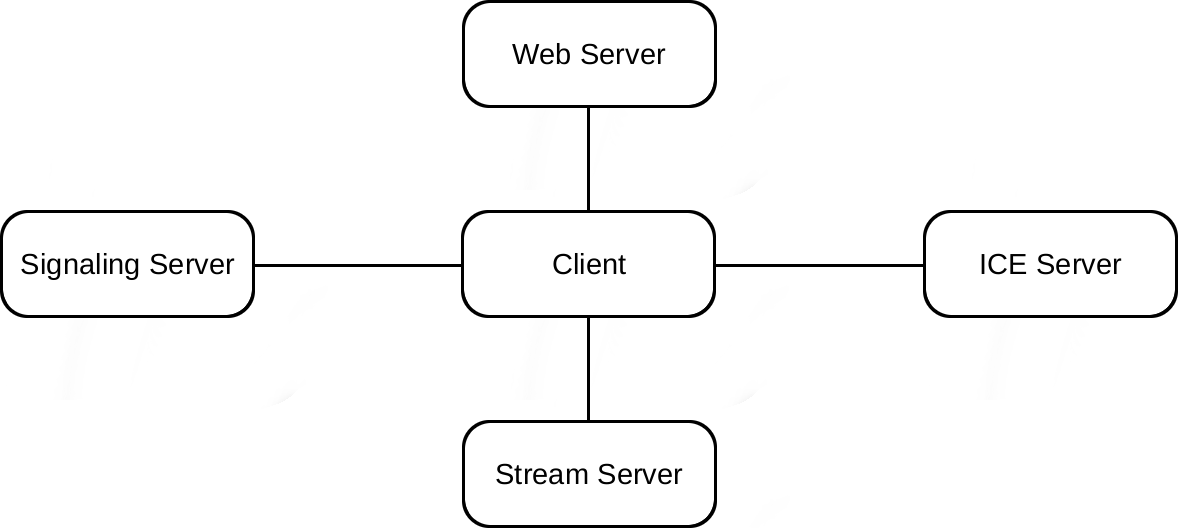
\includegraphics[width=0.55\textwidth]{figures/archs.png}
	\caption{System Modules}
\end{figure}

 The Web Server sends Web Pages, containing the other modules information, to the client, after this, the client contacts all the other modules. The ICE server will be used for \ac{NAT} traversal. The Stream Server will be used to record streams for further playback. The signaling server will be responsible for user and calls management. The web server will provide libraries to the client in order to interact with the other modules.  

\subsection{Implementation Proposal}
The infrastructure is composed by: Ice Server, Web Server, Stream Server, Signaling Server and Test Clients.

\begin{figure}[H]
	\centering
	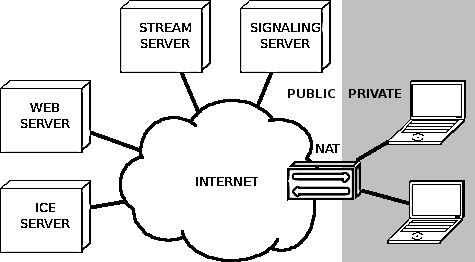
\includegraphics[width=0.55\textwidth]{figures/arch.png}
	\caption{System Architecture}
\end{figure}

Although the core infrastructure is important and crucial for the implementation of our web application, there is no preference for a specific software running on the web server. An important requirement for the Web Server is the WebSockets support, \emph{LAMP} server was considered, although the chosen technology for web development is \emph{Play Framework} with \emph{Java}, which has a more evident separation between \emph{Model}, \emph{View} and \emph{Controller} components.

For the signaling server there is also no preference between \ac{SIP} and \ac{XMPP}, as both support presence information feature. \ac{SigOfly} could be adopted as well but using it would be irrelevant for the final result of this project. For sake of simplicity and easy deployment the chosen platform chosen is the \emph{Ejabberd} \ac{XMPP} application server since it implements \cite{xep0206} which is crucial for web applications, \emph{Ejabberd}, as said before, is also the \ac{XMPP} server that implements more extensions. Initially, for simplicity, \emph{Ejabberd} will be configured as a single node instead a member of cluster. 

The streaming server will be \emph{Jitsi Videobridge} as \emph{Jitsi} team is working with \ac{WebRTC} and their code is open source.

The \ac{ICE} server is not required to be on our infrastructure as a public \ac{ICE} server could be used, if \ac{TURN} is used the network speed could drop due to resource share amongst other users. An \ac{ICE} server will be installed in order to prevent the influence of other users on our application.

On the client computers, both \emph{Mozilla Firefox} and \emph{Google Chrome} will be installed as web browsers. Libraries such as \emph{jQuery}, \emph{Bootstrap}, \emph{Strophe}, \emph{Modernizr} and \emph{TogetherJS} will be downloaded from the Web Server and executed on the client side.

\begin{figure}[H]
	\centering
	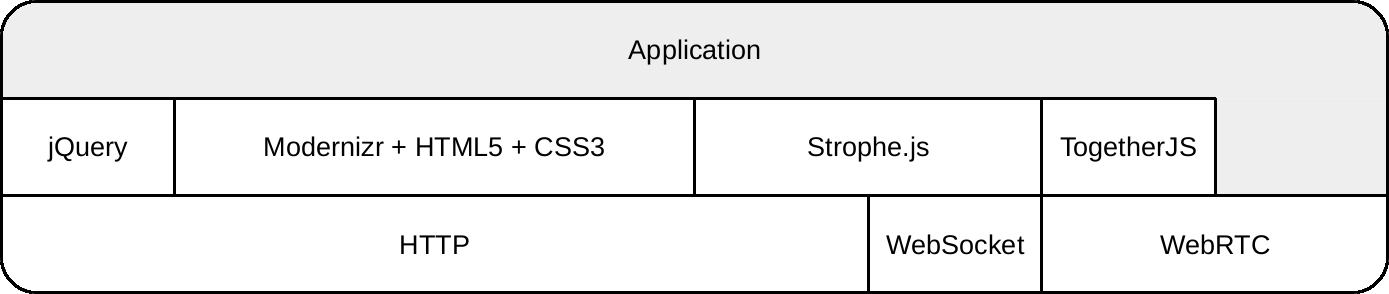
\includegraphics[width=0.95\textwidth]{figures/apparch.png}
	\caption{App Architecture}
\end{figure}

\emph{Modernizr} and \emph{jQuery} will ensure that our application is compatible with the most popular web browsers.

\emph{Bootstrap} will be used to make user interface more appellative and responsive. With \emph{bootstrap} it's quite easy to develop applications that adapt to mobile devices with different screen sizes.

\emph{Strophe} library will be essential to communicate with \ac{XMPP} server and clients.

\emph{TogetherJS} will be used for the collaborative component of our web application, other libraries were considered but, as said before, \emph{TogetherJS} does not implement object storage making the object storage implementation free.